\documentclass{amsart}
\usepackage{mathtools}
\usepackage{graphicx} % Required for inserting images
\usepackage{amsmath}
\usepackage{amssymb}

%%%%%%%%%%%%%%%%%%%%
\usepackage{tikz}
\usepackage{tikz-cd}

\usepackage{tikz-3dplot}
\usepackage{amsrefs}
\usepackage{pgfplots}
\usepackage{listings}
\usepackage{ulem}

\pgfplotsset{%
    compat=1.8,
    compat/show suggested version=false,
}

 

\usepackage{asypictureB}


\usetikzlibrary{calc,fadings,decorations.pathreplacing}

\usepackage[many]{tcolorbox}


%%%%%%%%%%%%%%%%%%%%%%%%%%%%%%%%%%%%%%%%%%%%%


\newtheorem{theorem}{Theorem}[section]
\newtheorem{proposition}[theorem]{Proposition}
\newtheorem{corollary}[theorem]{Corollary}
\newtheorem{lemma}[theorem]{Lemma}
\newtheorem{definition}[theorem]{Definition}
\theoremstyle{remark}
\newtheorem{example}[theorem]{Example}
\newtheorem{remark}[theorem]{Remark}
\renewcommand{\refname}{References}
\renewcommand{\abstractname}{Abstract}
\numberwithin{equation}{section}

\newcommand{\tc}{\textcolor{blue}}
\newcommand{\tcg}{\textcolor{green}}
\newcommand{\RR}{\mathbb{R}}
\newcommand{\CC}{\mathbb{C}}
\newcommand{\NN}{\mathbb{N}}
\newcommand{\PP}{\mathbb{P}}

\newcommand{\re}{\text{Re}~}
\newcommand{\im}{\text{Im}~}

\def\mclimits_#1{\limits_{\mathclap{#1}}}








\begin{document}
\title{The Gaussian Radon transform, Pad\'e approximants, and shape reconstruction}


\date{\today}

\author[M.~Derevyagin]{Maxim~Derevyagin}
\address{
MD,
Department of Mathematics\\
University of Connecticut\\
341 Mansfield Road, U-1009\\
Storrs, CT 06269–1009, USA}
\email{maksym.derevyagin@uconn.edu}

\author[A.~Sengupta]{Ambar~Sengupta}
\address{
AS,
Department of Mathematics\\
University of Connecticut\\
341 Mansfield Road, U–1009\\
Storrs, CT 0626–91009, USA}
\email{ambar.sengupta@uconn.edu}

\author[J.~Toman–Yih]{Jasper~Toman–Yih}
\address{
JT,
Department of Mathematics\\
University of Connecticut\\
341 Mansfield Road, U–1009\\
Storrs, CT 06269–1009, USA}
\email{jasper.toman–yih@uconn.edu}

\subjclass{Primary ????; Secondary ????.}
\keywords{????; ????; ????.}

\begin{abstract}
\tc{To be done later}
\end{abstract}

\maketitle

\section{Introduction}

Here is a sort of to-do list for whatever this document is:
\begin{itemize}
\item To write:
\begin{itemize}
\item \sout{Intro. Place discussion of Mathematica implementation and other numerical stuff into its own section.}
\item \sout{Intro. Discuss in the role of the Radon transform in proofs supporting the method, as well as its extension to the Gaussian transform.}
\item RT/GRT.\@ Work on notation for Gaussian measure. In particular $w$ and $\omega$ are too similar. Also the Euclidean norm is inconsistent when going from $\RR^n$ to $\RR^{n-1}$. We think the notation is understandble, but it might be more precise to disambiguate norms in different dimensions? Possible that they can all be dexribed in terms of a seminorm on some space in which each $\RR^n$ is embedded? 
\item RT/GRT.\@ Search for references on G slice theorem and G projection moments etc\ldots If none, congrats.
\item RT/GTT.\@ Expand background, historical context, etc\ldots
\item RT/GRT.\@ Swap sufficient working condition with Fubini condition in slice theorems.
\item Implementation. Output some figures from Mathematica. For example sample points, moment tables, and reconstructions.
\end{itemize}

\item To research:
\begin{itemize}
\item Everywhere. Provide examples for $n = 2, 3$ of as many results as we can.
\item GRT.\@ Domains of defintion, i.e. $GRT: L^2 \rightarrow L^2$ and such.
\item GRT.\@ Integration by parts formula for $GRT$ of $\partial f/\partial x_i$
\item Mathematica. Compute tables of GRT on monomials (polynomials). Do they look like anything? \sout{Compute GRT on Hermite polynomials?}
\item Mathematica. Implement Gaussian shape reconstruction method, try some example shapes. Clearly lay out the choices made: Series of expanding images, or compactified $\RR^n$? How to complexify points?
\end{itemize}
\end{itemize}

% And here is a section outline because I forget which one Maxim wanted:
% \begin{itemize}
% \item 
% \end{itemize}

The shape reconstruction method: In a 2005 paper, Annie Cuyt et. al. \cite{Cuyt05} proposed a method for shape reconstruction from moments, via Pade approximants to a multidimensional integral transform. Given a set of multivariate moments of some region $A$ in $\RR^n$, the method produces a pixel image approximating $A$. 

Suppose $A \subset \RR^n$ is suitably well behaved subset of $\RR^n$, and let $f(x)$ be its indicator function. In particular we may assume $f$ is measurable, has bounded support, and finite moments. The moment sequence gives Taylor coefficients for a certain holomorphic function with integral representation
\begin{align*}
    g(y) = \int_{\RR^n} \frac{f(x)}{1 + \langle x, y\rangle} ~dx = \sum_{\alpha \in \NN_0^n} \binom{|\alpha|}{\alpha} c_\alpha {(-y)}^\alpha.
\end{align*}
Thus the function $g(y)$ may be approximated to a certain degree of accuracy depending on the number of available moments.

At the same time $g$ can, in theory, be approximated by a multivarirate quadrature formula
\[
    \int_{\RR^n} \frac{f(x)}{1 + \langle x, y\rangle} ~dx
    = \sum_{i} \frac1{1+\langle x_i, y\rangle} f(x_i)
    = \sum_{i} w(x_i, y) f(x_i)
\]
Where the nodes $x_i$ lie, for example, on a cubic lattice. We can then sample a Pade approximant to $g$ at some sufficinetly large group of points $y = y_j$ forming a linear system of equations, from which we — again, at least in theory — solve for $f(x_i)$. If all goes well we have approximations of $f(x_i)$ on a node lattice, which can be turned into a pixel image of $A$.

For now we will gloss over the numerical discussion of quadrature and linear systems, taking for granted that such methods are applicable in at least some simple cases. Computational tests (to be included in, say, section 10) further support the validity of the method. Our focus will be on demonstrating that one can approximate $g$ by rational Pad\'e approximants constructed from moments. To this end we show that, when restricted to one dimensional subspaces, $g$ is equivalent to the Stieltjes transform of the Radon transform of $f$ at a fixed projection angle. 
\[
    g(z\omega) = \int_{-\infty}^\infty \frac{R_f(\omega,p)}{1 + zp}dp
\]
where $\omega \in S^{n-1}, z\in \RR$. Thus we are able to leverage the more well understood properties of these univariate transforms. 

In particular, the ``projection moments'' of $R_f(\omega, p)$ in any fixed direction $\omega$, may be computed from the multivariate moments of $f$. Further, it can be shown that Pad\'e approximants to a moment sequence converge to the Stieltjes transform, and thus to $g$. Returning to shape reconstruction, it then follows that one can approximate $g$ at various sample points $y_j = z_j\omega_j$ via Pad\'e approximants on linear subspaces at a selection of angles $\omega$.

Now let us briefly discuss our proposed modification to the shape reconstruction moments, the theoretical complications and computational considerations. Essentially what we propose is to recreate the method with a Gaussian measure applied, thus allowing for convergence on a larger class of regions $A$. In particular, the proposed method would apply to unbounded regions. 

Here we will briefly discuss the potential challenges that this proposed method presents, which we address more carefully in sections 5 through 8. First and foremost instead of classical moments, we are now given a Gaussian moment sequence — that is, moments with respect to the standard Gaussian measure on $\RR^n$. On the other end, the reconstructed region may be recovered as normal by simply inverting the Gaussian weight. 

From a theoretical standpoint, proving the validity of the proposed method presents a few challenges. Firstly, even a quick glance at the classical literature tells us that moment problems on bounded domains are substantially better behaved than their unbounded counterparts. Whereas all continuous moment problems on a bounded interval are determinate, we now have the potential to run in to indeterminate problems. This turns out to be not so much of a challenge, since we can guarentee determinacy in a Gaussian-weighted $L^2$ completion of the space of polynomials. This of course includes our primary use case: indicator functions. 

Secondly, we must address the effect of the proposed modifications on the Radon and Stieltjes transforms. We will define the Gaussian Radon transform, which has been the subject of decades of study in its own right. We build off of this previous work, together with some (possibly) new results, to validate our method. The Stieltjes transform in the Gaussian context is likewise not a significant complication. The main complication here arrises from the claim that our method should apply to unbounded regions:

A final major complication arrises when we try to define the function $g(y)$. From the integral representation
\[
    g(y) = \int_{\RR^n} \frac{f(x)}{1 + \langle x, y\rangle} ~dx,
\]
one can start to see a problem: If $f(x)$ has unbounded support $g(y)$ has the potential to not converge for any $y \in \RR^n$. In particular $g(y)$ may not exist in a neighborhood of $0$, meaning our series expansion and thus the explicit conection to moments, may be broken. We need now to consider $g$ as a function on some non-real domain. Here, as it turns out, Pade approximants can be computed from moments which approximate $g$ on, for example, a half space. The convergence of these approximants is tied to the question determinacy of the moment problem, which as mentioned above is not difficult to resolve. Thus we simply take sample points avoiding the problematic real space and — at least in theory — the method is validated.


% But if $x$ ranges over $\RR^n$
% \begin{align*}
%     1 + \langle x, y \rangle &= 0 \\
%     \langle x, y \rangle &= -1 \\
% \end{align*}
% The integral is always nonconvergent. 

% An outline of my "research" is as follows
% \begin{enumerate}
% \item Krawtchouk polynomials
% \item The Radon Transform and Gaussian Radon Transform
% \item Discrete Radon Transforms
% \item Shape reconstruction
% \end{enumerate}

% The shape reconstruction method (ref cuyt) is summarized as follows
% \begin{enumerate}
% \item Suppose a certain number of multivariate moments are given for an unknown shape $A$ of bounded support.
% \item From the moments one constructs Cuyt's multivariate pade approximants to multivairate Markov transform of $A$.
% \item The multivariate Markov transform is simultaneously approximated by a cubature formula with nodes on a cubic or near cubic latice.
% \item By equating these two approximants — and tuning their order appropriately — we form a linear system which can, in theory, be solved to approximate $A$ at each latice node. After quantization we have a pixel image approximating $A$
% \end{enumerate}
% Since a key property of Cuyt's multivariate Pade approximants was their equivalence to univariate approximants to the radon transform when restricted to one dimensional subspaces, we chose to bypass the multivariate approximants. We agknowledged the possibility that some computational efficiency is gained by computing a single multivariate approximant over many univariate ones.

% Here's a slightly more verbose outline of the method:

% Let $A$ be a bounded subset of $\RR^n$, and $f(x)$ its indicator function. Since $A$ is bounded, $f$ has finite moments 
% \[
%     c_\alpha = \int_{\RR^n} f(x) x^\alpha ~dx < \infty, \qquad \alpha \in \NN_0^n
% \]
% Now suppose we are given the moment sequence $c_\alpha$. The goal is to reconstruct $f$ — and thus $A$. Our strategy is to pass through a generating function: The moment sequence can be seen as series coefficients for a certain holomorphic function $g(z)$, called the Markov transform of $f$. 

\newpage
\section{Notation}
First recall the conventional multiindex notation. Let $\NN_0$ denote the nonnegative integers. A multiindex $\alpha = (\alpha_1, \alpha_2, \ldots, \alpha_n) \in \NN_0^n$ is an $n$-tuple of nonnegative integers. The degree of a multiindex is $|\alpha| = \alpha_1 + \alpha_2 + \cdots + \alpha_n$. Multivariate exponentiation is defined as follows. For $x = (x_1, x_2, \ldots, x_n) \in \RR^n$,
\[
    x^\alpha = x_1^{\alpha_1}x_2^{\alpha_2} \cdots x_n^{\alpha_n}.
\]
The multinomial formula gives a convenient expansion for multinomial powers. Let $k \in \NN_0$. Then
\[
    {(b_1 + b_2 + \cdots + b_n)}^k = \sum_{|\alpha| = k} \binom{k}{\alpha} b^\alpha
\] 
where the multinomial coefficients are defined
\[
    \binom{k}{\alpha} = \frac{k!}{\alpha_1! \alpha_2! \cdots \alpha_n!}.
\]
Note that the multinomial expansion sums over all multiindeces $\alpha \in \NN_0^n$ of degree $k$.

We denote the standard euclidean inner product
\[
    \langle x,y \rangle = x_1y_1 + x_2y_2 + \cdots x_n y_n
\]
where $y = (y_1, y_2, \ldots, y_n) \in \RR^n$. When discussing hyperplanes in $\RR^n$ we index them by a unit normal vector, $\omega \in S^{n-1}$, and distance from origin $-\infty < p < \infty$, and we write for example $\langle x, \omega \rangle = p$. Note that $\langle x, -\omega \rangle = p$ is the same hyperplane. It is perhaps more correct, in later defining the Radon and Gaussian Radon transforms, to identify these indexes and define the transforms over a projective space. We omit this discussion as it is not relevant within the scope of this work.
\begin{figure}
    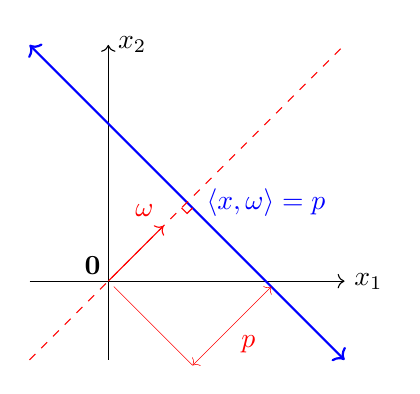
\begin{tikzpicture}[plane/.style={<->,thick,blue},
        vector/.style={->,red},
        axis/.style={->,black}]
    %draw axes
    \draw[axis] (-1,0) -- (3,0) node[anchor=west]{$x_1$};
    \node at (-.2,.2) {$\mathbf{0}$};
    \draw[axis] (0,-1) -- (0,3) node[anchor=west]{$x_2$};
    %draw plane
    \draw[plane] (-1, 3) -- (3, -1) node[midway, right]{~$\langle x, \omega\rangle = p$};
    %draw projection angle and orthogonal vector
    \draw[red,dashed] (-1,-1) -- (3,3);
    \def\ra{.07};
    \draw[red] (1-\ra, 1-\ra) -- (1,1-2*\ra) -- (1+\ra,1-\ra);
    \draw[vector] (0,0) -- (0.7,0.7) node[above left]{$\omega$};
    %draw extension line
    \draw[very thin, red] (\ra, -\ra) -- (1+\ra, -1-\ra);
    \draw[<->,very thin, red] (1+\ra, -1-\ra) -- (2+\ra, -\ra) node[midway,below right]{$p$};
    \end{tikzpicture}
\end{figure}

Unless otherwise indicated all measures are Euclidean measures, that is the Borel measure assocciated with the standard Euclidean metric on a given space. In particular the Euclidean measure on a hyperplane of $\RR^n$ is equivalent to the Euclidean measure on $\RR^{n-1}$. We chose for convenience to denote measures by their associated variable such as $dx$, $dp$, $dz$, and others. It should be stated that this notation, while uniform, is context dependent. For example in the integrals
\[
    \int_{\RR^n}~dx \qquad \text{and} \qquad \int_{\langle x, \omega\rangle = p} ~dx,
\]
the measure $dx$ is to be understood as the $n$-dimensional and $(n-1)$-dimensional Euclidean measure respectively.

\newpage
\section{Classical and Multivariate Moments}
Let $f(x)$ be a measurable function on $\RR$. For $k \in \NN_0$, define the $k$th moment of $f$ as
\[
    c_k = \int_{-\infty}^\infty f(x)x^k ~dx.
\]
The sequence ${(c_k)}_{k \in \NN_0}$ is called a moment sequence or a moment problem, and the function $f$ is called a solution to the moment problem. Loosly speaking a moment problem poses the question: Under given constraints (e.g.\ domain, continuity, etc\ldots), to what extent can one determine the solution $f$ from its moments?

The classical study of moment problems is divided into three cases depending on the domain: 
\begin{enumerate}
\item Markov (or Haussdorf) moment problems for bounded domains (i.e.\ the unit interval), 
\item Stieltjes moment problems for one-sided unbounded domains (i.e.\ the positive real line), and 
\item Hamburger moment problems for bi-infinite domains (i.e.\ the real line).
\end{enumerate}

There are two natural questions one can ask about a moment problem:
\begin{enumerate}
\item Solvability: Does a solution $f$ exist possessing the given moments?
\item Determinacy: Is a solution unique? If not, what can be said about the set of solutions?
\end{enumerate}
In the classical cases (Markov, Stieltjes, Hamburger) these questions have been resolved. Precise conditions for solvable and determinate moment problems exist, and the nature of solution sets to indeterminate moment problems are well understood. For instance, in the class of continuous functions on the unit interval, all solvable moments problems are determinate. However many classes of generalized moment problems remain in active study.

In particular let us discuss multivariate moment problems. Let $f(x)$ be a measureable function now on $\RR^n$. For $\alpha \in \NN_0^n$, define the $\alpha$th multivariate moment of $f$ as 
\[
    c_\alpha = \int_{\RR^n} f(x)x^\alpha ~ dx.
\]
The moment sequence ${(c_\alpha)}_{\alpha \in \NN_0^n}$ is now multiindexed. No precise general conditions are known for the solvability or determinacy of multivariate moment problems. However some sufficient conditions have been discovered by leveraging classical moment problem theory~\cite{Pete82}.


\newpage
\section{Gaussian Functions and Gaussian Measures}
Let $w(p) : \RR \rightarrow \RR$  be the standard Gaussian density on $\RR$,
\[
    w(p) = \frac1{\sqrt{2\pi}}e^{\frac{-p^2}2}
\]
and $w_n(x) : \RR^n \rightarrow \RR$ the standard Gaussian density on $\RR^n$,
\[
    w_n(x) = {(2\pi)}^{-\frac n2} e^{\frac{-\|x\|^2}2}.
\]
Note that $w = w_1$.

A relationship between the univariate and multivariate Gaussian densities can be seen as follows: Let $x, y \in \RR^n$, $n \geq 2$. Suppose $y = p\omega$ where $\omega \in S^1$ and $p \in \RR$, so that $p\omega$ is the orthogonal projection of $x$ onto the span of $y$. Then the Pythagorean relation,
\[
    \|x\|^2 = \|x - p\omega\|^2 + \|p\omega\|^2 = \|x - p\omega\|^2 + p^2
\]
implies that
\begin{align*}
    w_n(x) 
    &= {(2\pi)}^{-\frac n2} e^{\frac{-\|x\|^2}2} \\
    &= {(2\pi)}^{-\frac{n-1}2} e^{\frac{-\|x - p\omega\|^2}2} {(2\pi)}^{-\frac12} e^{\frac{-p^2}2} \\
    &= w_{n-1}(x - p\omega)w(p)
\end{align*}
The equation
\begin{equation}\label{eq:gaussPythag}
    w_n(x) = w_{n-1}(x - p\omega)w(p)
\end{equation}
is in some respect the defining property of the Gaussian measure defined below. Indeed if $x = (x_1, x_2, \ldots, x_n)$, by repeated application of (\ref{eq:gaussPythag}) one can write the decomposition
\[
    w_n(x) = \prod_{k = 1}^n w(x_k).
\]
Thus the $w_n(x)$ is the product of $n$ copies of $w$. The standard Gaussian measure $\gamma^n$ is thus a measure whose cardinal projections are standard Gaussian measures.

\begin{definition}
Let $\gamma^n$ be a the Borel measure on $\RR^n$ with density $w_n$,
\[
    \int_{\RR^n} f(x) d\gamma^n = \int_{\RR^n} f(x) w_n(x) ~dx.
\]
We call $\gamma^n$ the standard Gaussian measure. More generally, for mean $a \in \RR^n$, and variance $\sigma > 0$, the following $\gamma^{n}_{a, \sigma^2}$ are Gaussian measures,
\begin{align*}
    \int_{\RR^n} f(x) d\gamma^n_{a,\sigma^2}
    &= \frac{{(2\pi)}^{-\frac n2}}{\sigma}  \int_{\RR^n} f(x) e^{-\frac{\|x - a\|^2}{2\sigma^2}} ~dx \\
    &= \int_{\RR^n} f(\sigma x + a) d\gamma^n
\end{align*}
(Most general defn of Gaussian measures includes degenerate $\delta$ functions, and any product of Gaussian measures).
\end{definition}



% In this sense the GRT is defined
% \[
%     GR_f(\omega, p) = \int_{\langle x, \omega \rangle = p} f(x) d\gamma^{n-1}
% \]
% or equivalently
% \[
%     GR_f(\omega, p) \frac{d\gamma}{dp} = R_g(\omega, p), \quad g(x) := g(x) \frac{d\gamma^n}{dx}
% \]
% and the GRT slice theorem takes the form
% \[
%     \int_{-\infty}^\infty GR_f(\omega, p) d\gamma = \int_{\RR^n} f(x) d\gamma^n
% \]


% \begin{align*}
%     GR_f(\omega, p) = \int_{\langle x, \omega \rangle = p} x^\alpha d\gamma^{n-1}
% \end{align*}
 
% \begin{align*}
    
% \end{align*}

\newpage
\section{Basics of the Radon and Gaussian Radon transforms}

Let $f$ be a multivariable function on the $n$-dimensional Euclidean space $\RR^n$. We imagine taking ``slices'' of $f$ by restricting it to a $(n-1)$-dimensional hyperplane $\Lambda$. These hyperplanes form the domain of the Radon Transform. More precisely, the Radon Transform associates each slice with a corresponding integral
\[
    R_f(\Lambda) = \int_{\Lambda} f(x) ~dx,
\]
which can be thought of as a $(n-1)$-dimensional measurement of $f$. To be more precise we parametrize the collection of hyperplanes $\Lambda$ by normal vector, $\omega \in S^{n-1}$, and (signed) distance from the origin $-\infty < p < \infty$. Indeed any hyperplane can be described in the form $\Lambda = \{x \in \RR^n: \langle x, \omega\rangle = p\}$. As mentioned, there is a slight inconsistency in these definitions where a hyperplane $\Lambda$ can be indexed by both $\langle \omega, x \rangle = p$ and $\langle -\omega, x \rangle = -p$. This difference is inconsequential for our purposes so we choose the latter for clarity.

The Radon transform~\cite{Helg65} (RT) is a thing that I will discuss the history of, with references, in this paragraph. The transform gets its name from Johann Radon, whose first defined the tranform in the form below in 1917, although a similar transform was introduced by Paul Funk in 1911~\cite{????}. It is interesting to note that the primary application of the RT in medical imaging (CT scans) was not invented for another half century.

\begin{definition}
    Let $f$ be a nonnegative measurable function on $\mathbb{R}^n$. The \textbf{Radon transform} $R_f : S^{n-1} \times \RR \rightarrow \RR$ of $f$ is a function which, given a unit vector $\omega \in \RR^n$ and $-\infty < p < \infty$, is defined as
    \[
        R_f(\omega, p) = \int\mclimits_{\langle x, \omega \rangle = p} f(x) ~dx,
    \]
    provided the integral converges.
\end{definition}

\begin{example}
For computation it is convenient to write the Radon Transform with an explicit isometric parameterization $x(t)$ of the hyperplane $\langle x, \omega\rangle = p$. In particular we note that there exists a map $x : \RR^{n-1} \longrightarrow \RR^n$ such that $x(0) = p\omega$ and
\[
    R_f(\omega, p) = \int_{\RR^{n-1}} f(x(t)) dt.
\]

For reference let's specify an hyperplane parameterization for the $n=2$ case. In $\RR^2$ often we identify $\omega$ with the angle $0 \leq \theta < 2\pi$ such that $\omega = (\cos \theta, \sin \theta)$. We define $x(t)$ by
\begin{align*}
    x(t) = (t \sin \theta + p \cos \theta, -t \cos \theta + p \sin \theta), \qquad -\infty < t < \infty.
\end{align*}
It is not difficult to show that $x(0) = p\omega$, $\langle x(t), \omega \rangle = p$, and most importantly
\[
    R_f(\omega, p) = \int_{-\infty}^\infty f(t \sin \theta + p \cos \theta, -t \cos \theta + p \sin \theta)~dt
\]
\end{example}

Our main addition to previous work will be the use of a modified RT, the Gaussian Radon transform (GRT). This transform is very similar to the RT, but the inclusion of a Gaussian density $w_{n-1}(x)$ in the integral allows for convergence on a larger class of functions $f$. In a broader context the Gaussian Radon transform also has the advantages of generalizng to infite dimensional Hilbert spaces~\cite{Seng14} (on which the Lebesgue measure is not defined), as well as having a natural probabilistic interpretation.

% Recall $w_{n-1}(x) = (2\pi)^{-n/2}\exp(-\|x\|^2/2)$

\begin{definition}
The \textbf{Gaussian Radon transform} $GR_f : S^{n-1} \times \RR \rightarrow \RR$ of $f$ is defined similarly to the RT.\@ Given $\omega \in S^{n-1}$ and $-\infty < p < \infty$, the GRT is
\[
    GR_f(\omega, p) = 
    \int\mclimits_{\langle x, \omega \rangle = p} f(x) w_{n-1}(x - p\omega) ~dx.
\]
provided the integral converges. Note the Gaussian density 
\[
    w_{n-1}(x - p\omega) = {(2\pi)}^{-(n-1)/2}e^{-\|x - p\omega\|^2/2}
\] 
is centered on the point of the hyperplane closest to the origin.
\end{definition}

\begin{figure}[h]
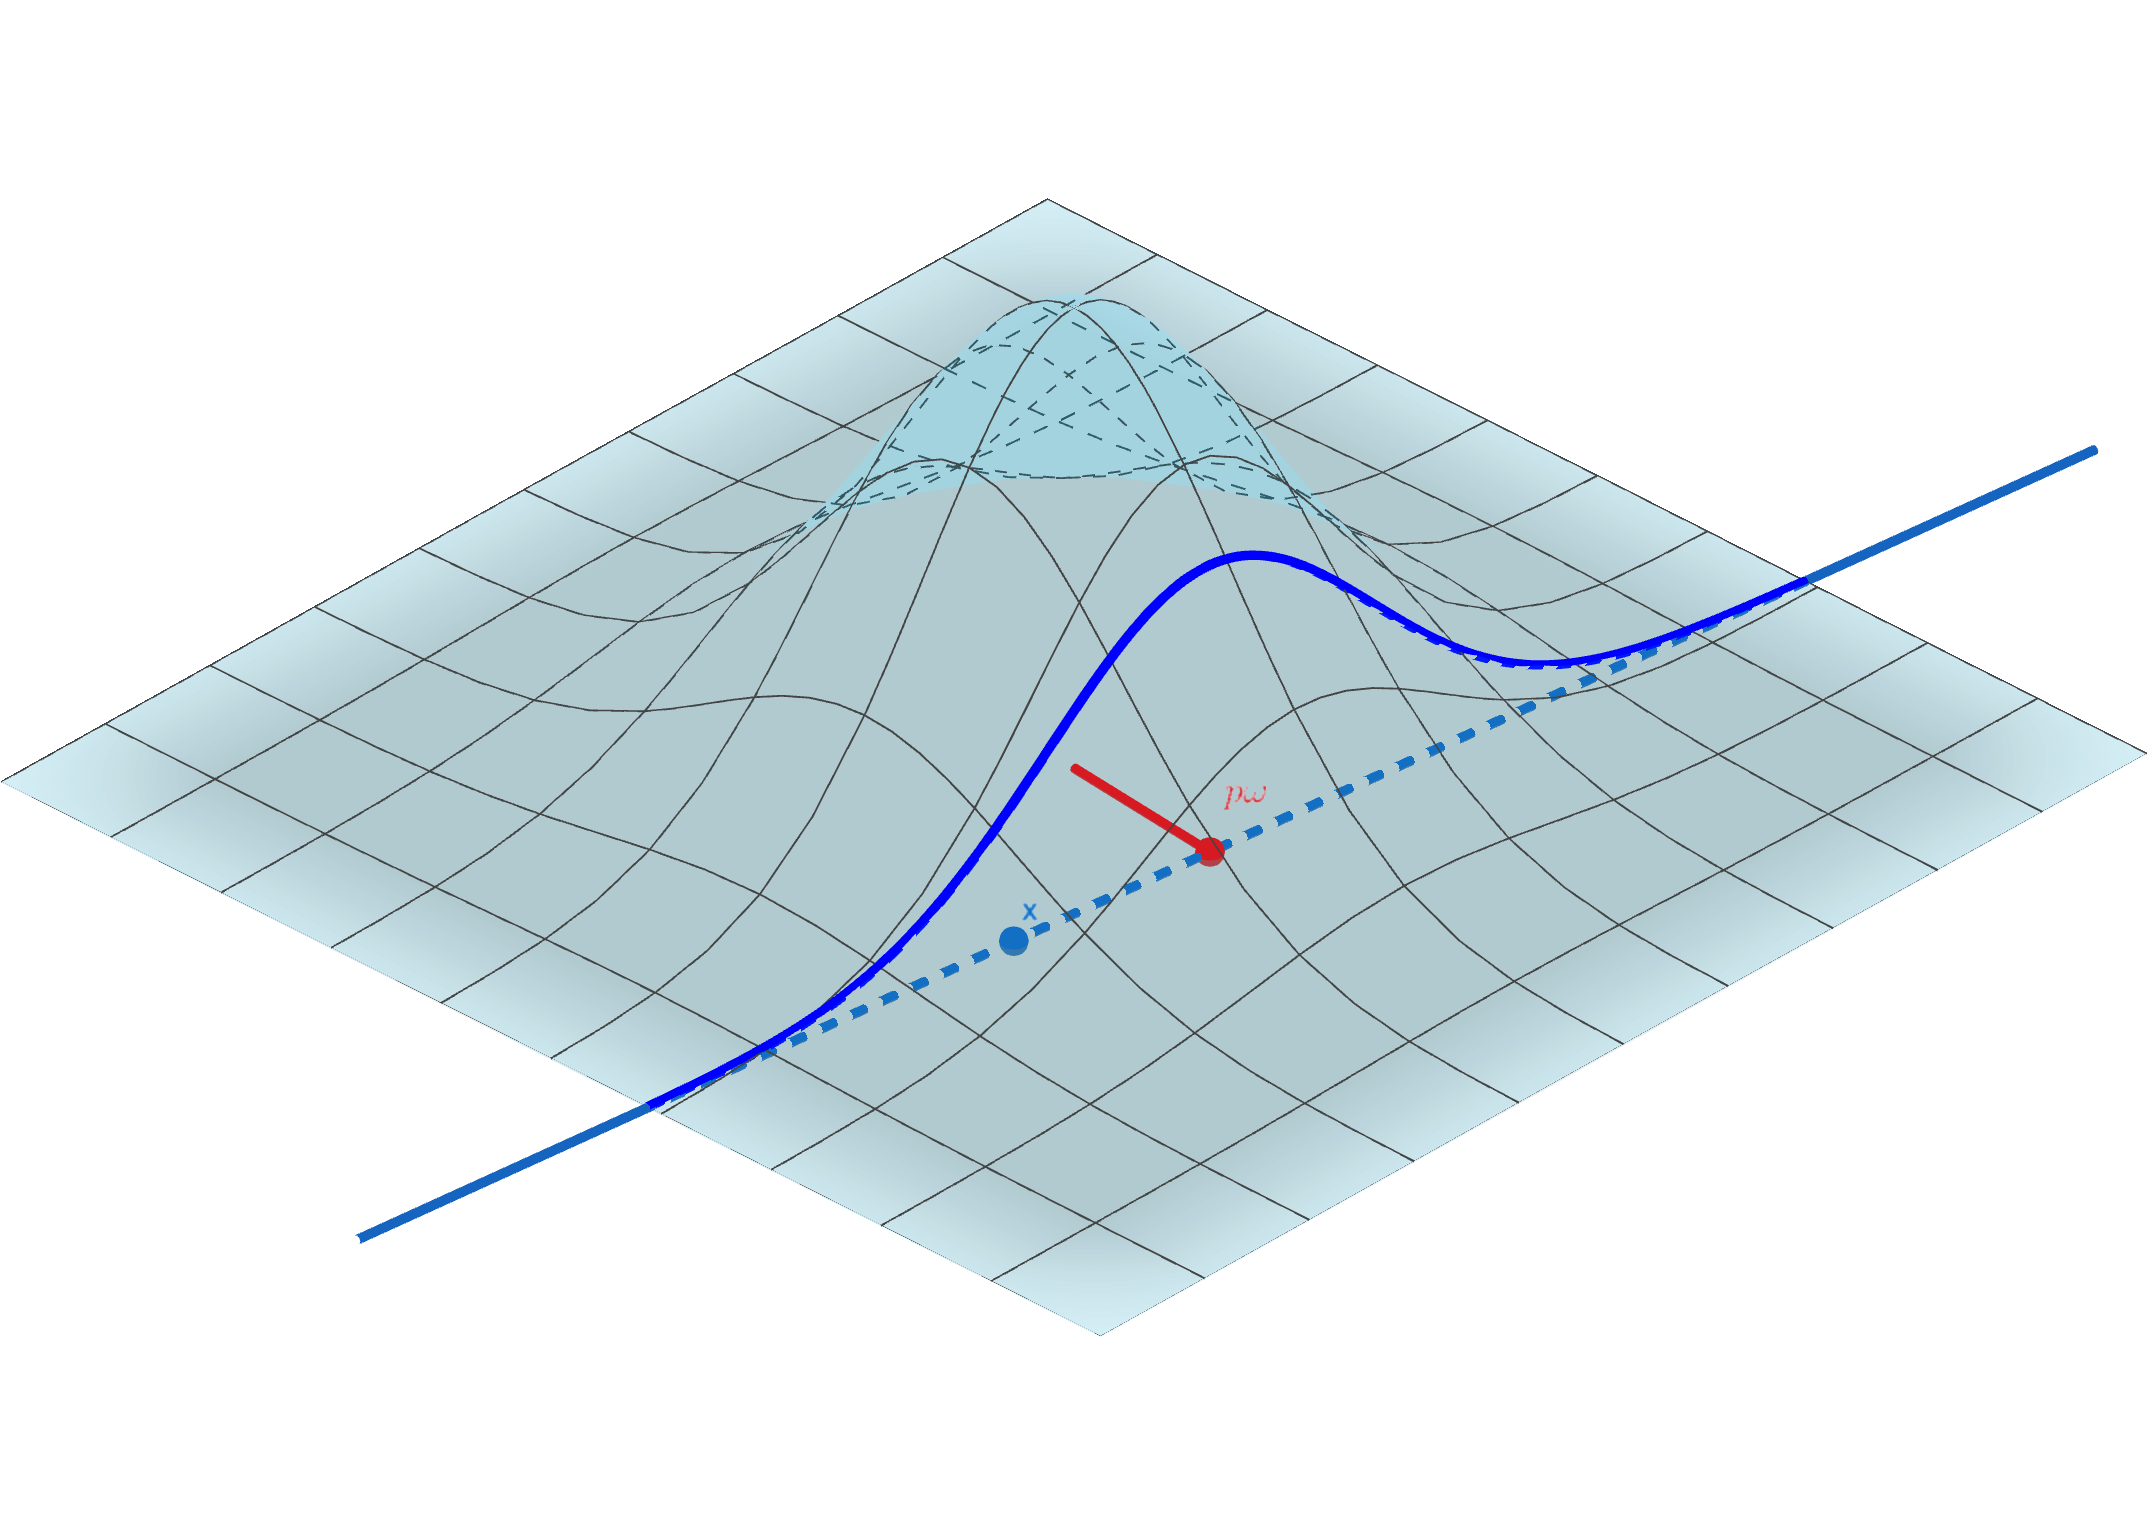
\includegraphics[width=0.7\textwidth]{geogebra-export.png}
\end{figure}

\begin{remark}
It may be helpful to understand the GRT as a simple modification of the RT with respect to a Gaussian measure on $\RR^n$. Let $g(x) := f(x)w_n(x)$. The RT of $g$ can be rewritten
\begin{align*}
    \int\mclimits_{\langle x, \omega \rangle = p} f(x) w_n(x) ~dx
    &= \int\mclimits_{\langle x, \omega \rangle = p} f(x) w_{n-1}(x) ~dx~ w(p),
\end{align*}
where we used the Pythagorean relation $\|x\|^2 = \|x - p\omega\|^2 + \|p\omega\|^2$. Since $\omega$ is a unit vector, $\|p\omega\|^2 = p^2$. In short, we have proved the formula
\begin{equation}
    \label{eq:GRTPythag}
    R_g(\omega, p) = GR_f(\omega, p) w(p), \qquad g(x) := f(x)w_n(x).
\end{equation}
The relation above provides decent intuition for the GRT, and is also a useful tool proving some basic properties of the transform.
\end{remark}

\begin{example}
If $x(t):\RR^{n-1} \longrightarrow \RR^n$ is a parametrization of $\langle x, \omega\rangle = p$ as described above, then
\[
    GR_f(\omega, p) = \int_{\RR^{n-1}}f(x(t)) w(t) dt
\]
In particular for $f:\RR^2 \rightarrow \RR$
\[
    GR_f(\omega, p) = \int_{-\infty}^\infty f(t \sin \theta + p \cos \theta, -t \cos \theta + p \sin \theta) w(t)~dt
\]
where $\omega = (\cos \theta, \sin \theta)$.
\end{example}

Now imagine sweeping a hyperplanar ``slice'' across $\RR^n$. As a function of $p$, the RT $R(\omega, p)$ can be seen as a projection of $f$ onto the linear subspace spanned by $\omega$. It is not surprising that integrating this projection over $-\infty < p < \infty$ we get the same result as the $n$-fold integral of $f$ over $\RR^n$.
\[
    \int_{-\infty}^\infty R(\omega, p) ~dp = \int_{\RR^n} f(x) ~dx
\]
The so called ``slice theorem'' further generalizes this observation.
% In fact, the following "slice theorem" gives a formula for integrating a projection against any weighting function $F(p)$, assuming the integral converges. 
\begin{proposition}[Slice Theorem]
    If $\int_{\mathbb{R}^n} |f(x) F(\langle x, \omega \rangle)| dx < \infty$ then
    \begin{align}
        \label{eq:ST}
        \int_{-\infty}^\infty R_f(\omega, p) F(p) dp 
        % &= \int_{-\infty}^\infty \int_{\langle x, \omega \rangle = p} f(x) F(p) ~d\mu(x) ~dp 
        &= \int_{\mathbb{R}^n} f(x) F(\langle x, \omega \rangle) dx.
    \end{align}
\end{proposition}

\begin{proof}
Inserting the definition of the RT, the left side is
\[
    \int_{-\infty}^\infty \int\mclimits_{\langle x, \omega \rangle = p} f(x) ~dx~ F(p) ~dp 
    = \int_{-\infty}^\infty \int\mclimits_{\langle x, \omega \rangle = p} f(x) F(\langle x, \omega \rangle) ~dx dp.
\]
Up to a rigid transformation (under which the Euclidean measures are invariant) this is essentially an itterated integral over $\RR$ and $\RR^{n-1}$. Thus given the integrability requirement, Fubini's theorem applies and the theorem is proved.
\end{proof}

\begin{remark}
We can specify various conditions for convergence. If $F(p)$ is bounded then $\int |f(x)| dx < \infty$ suffices for convergence. If $f$ is continuous with compact support then $F(p)$ only needs to be integrable.  
\end{remark}

If $F(p) = e^{-ip}$ and $f(x)$ is such that $\int_{-\infty}^\infty R_f(\omega, p) dp < \infty$ then (\ref{eq:ST}) becomes the well known Fourier slice theorem
\[
    \int_{-\infty}^\infty R_f(\omega, p) e^{-ip} ~dp
    = \int_{\mathbb{R}^n} f(x) e^{-i\langle x, \omega\rangle} ~dx,
\]
which is often articulated as saying that the $1$-dimensional Fourier transform of the Radon transform is the $n$-dimenstional Fourier transform of $f$.

An early and natural question in the study of the RT is that of inversion. Radon himself derived the ``Radon inversion formula''~\cite{Rado17}~\cite{Rado86}, which is often proved via the above Fourier slice theorem. The groundbreaking inversion formula is the basis for what, in application, called ``filtered backpropogation''.

If one is interested in inverting the RT then a prerequisite consern is of course: Is the transform injective? The answer clearly depends on what space we draw the function $f$ from. Radon~\cite{Rado17}~\cite{Rado86} provides a set of sufficient regularity conditions such that the RT is invertible. Other similar results followed \cite{????}. On the other hand counterexamples have been constructed by, for example, Lawrence Zalcman~\cite{Zalc82}, of continuous and nontrivial functions for which the RT is identically zero.

By way of the relation (\ref{eq:GRTPythag}) we can prove an analagous slice theorem for the GRT.\@
\begin{theorem}[Gaussian Slice Theorem] If $\int_{\mathbb{R}^n} |f(x) F(\langle x, \omega\rangle) w_n(x)| dx < \infty$ then
\begin{equation}\label{eq:GST}
    \int_{-\infty}^\infty GR_f(\omega, p)F(p) w(p) ~dp
    = \int_{\mathbb{R}^n}f(x) F(\langle x, \omega\rangle) w_n(x) ~dx. 
\end{equation}
\begin{remark}
Whatever conditions are sufficient for convergence in (\ref{eq:ST}) are then sufficient conditions to be checked for $f(x)w_n(x)$ and $F(p)w(p)$. For example it is sufficient that $f \in L^1(\RR^n, w_n)$ and $F \in L^\infty$. Note in particular that this applies bounded functions of potentially unbounded support, and to all polynomials $f \in \RR[x]$.
\end{remark}
\end{theorem}
\begin{proof}
From (\ref{eq:GRTPythag})
\[
    \int_{-\infty}^\infty GR_f(\omega, p)F(p) w(p) ~dp 
    = \int_{-\infty}^\infty R_g(\omega, p) F(p) ~dp
\]
where $g(x) = f(x)e^{-\|x\|^2/2}$. Then applying the slice theorem:
\[
    \int_{-\infty}^\infty R_g(\omega, p) F(p) ~dp 
    = \int_{\RR^n} f(x)F(\langle x, \omega \rangle) w_n(x) ~dx,
\]
completing the proof.
\end{proof}

% \begin{remark}
%     For an equivalent 
% \end{remark}

As an applications of the slice theorems going forward, we first show that, fixing $\omega$, the $k$th projection moment at $\omega$ can be written as a weighted sum of the degree $k$ multivariate moments of $f$. 
\begin{proposition}
    Let $c_\alpha (\omega) = \int_{-\infty}^\infty R_f(\omega, p) p^k dp$ be the projection moments of $f$ at a fixed $\omega$, and $c_\alpha$ the multivariate moments of $f$. Then
    \[
        c_k(\omega) = \sum_{|\alpha| = k}\binom{k}{\alpha} \omega^\alpha c_\alpha
    \]
    where $\binom{k}{\alpha} = \frac{k!}{\alpha_1! \alpha_2! \cdots \alpha_n!}$ are multinomial coefficients.
\end{proposition}
\begin{proof}
By the slice theorem (\ref{eq:ST}) with $F(p) = p^k$,
\[
    \int_{-\infty}^\infty R_f(\omega, p) p^k ~dp 
    = \int_{\RR^n} f(x) \langle x, \omega \rangle^k ~dx.
\]
Now $\langle x, \omega \rangle^k = {(x_1 \omega_1 + \cdots + x_n \omega_n)}^k$ has the multinomial expansion
\[
    \langle x, \omega \rangle^k = \sum_{|\alpha| = k}\binom{k}{\alpha} x^\alpha\omega^\alpha.
\]
Thus after a bit of rearranging we get
\begin{align*}
    \int_{\RR^n} f(x) \langle x, \omega \rangle^k ~dx
    &= \int_{\RR^n} f(x) \sum_{|\alpha| = k}\binom{k}{\alpha} x^\alpha \omega^\alpha ~dx \\
    &= \sum_{|\alpha| = k}\binom{k}{\alpha} \omega^\alpha \int_{\RR^n} f(x) x^\alpha ~dx,
\end{align*}
where the integrands are precisely the $k$th degree multivariate moments of $f$.
\end{proof}
% \begin{align*}
%     c_k(\omega) &:= \int_{-\infty}^\infty R_f(\omega, p) p^k dp \\
%     &= \int_{\RR^n} f(x) \langle x, \omega \rangle^k dx \\
%     &= \sum_{|\alpha| = k}\binom{k}{\alpha} \omega^\alpha \int_{\RR^n} f(x) x^\alpha dx
%     =: \sum_{|\alpha| = k}\binom{k}{\alpha} \omega^\alpha c_\alpha
% \end{align*}
Similarly, moments of the GRT (Gaussian projection moments) can be expressed in terms of multivariate gaussian moments.
\begin{proposition}
Let $c_k^G(\omega) = \int_{-\infty}^\infty GR_f(\omega, p) p^k w(p) dp$ be the Gaussian weighted moments of the GRT of $f$ at a fixed $\omega$. Let $c^G_\alpha = \int_{\RR^n} f(x) w_n(x) x^\alpha dx$ be the Gaussian weighted multivariate moments of $f$. Then
\[
    c^G_k(\omega) = \sum_{|\alpha| = k}\binom{k}{\alpha} \omega^\alpha c^G_\alpha.
\]
\end{proposition}

\begin{proof}
The proof follows as it did for the RT.\@ This time we apply the GRT slice theorem (\ref{eq:GST}) with $F(p) = p^k$, 
\begin{align*}
    \int_{-\infty}^\infty GR_f(\omega, p) p^k w(p) ~dp
    &= \int_{\RR^n} f(x) \langle x, \omega \rangle^k w_n(x) ~dx
\end{align*}
Again we use the multinomial expansion of $\langle x, \omega\rangle^n$ and rearange:
\[
    \int_{\RR^n} f(x) \langle x, \omega \rangle^k w_n(x) ~dx
    = \sum_{|\alpha| = k} \binom{k}{\alpha} \omega^\alpha \int_{\RR^n} f(x) w_n(x)x^\alpha dx. 
\]
Thus
\[
    c^G(\omega) = \sum_{|\alpha| = k} \binom{k}{\alpha} \omega^\alpha c^G_\alpha.
\]
% \begin{align*}
%     c_k^G(\omega) &:= \int_{-\infty}^\infty GR_f(\omega, p) p^k e^{-p^2/2} dp \\
%     &= \int_{\RR^n} f(x) e^{-\|x\|^2/2}\langle x, \omega\rangle^k dx \\
%     &= \sum_{|\alpha| = k} \binom{k}{\alpha} \omega^\alpha \int_{\RR^n} f(x) e^{-\|x\|^2/2}x^\alpha dx 
%     =: \sum_{|\alpha| = k} \binom{k}{\alpha} \omega^\alpha c_\alpha^G
% \end{align*}
\end{proof}

% \tc{Is this really the assumption we want? Check more carefully.}
% For our purposes it will suffice to assume that $f(x) e^{-\|x\|^2/2}$ is bounded and $\int_{-\infty}^\infty |F(p)e^{p^2/2}| dp < \infty$.

% \tc{Or is it this?}
% One case of interest: Suppose $|f(x)| \leq M$. Then $|GR_f(\omega, p)| \leq M \sqrt{2\pi}$, and the slice theorem holds if $F(p)$ is integrable.
\newpage
\section{The Markov and Hamburger Transforms}
Let $\mu$ be a Borel measure with infinite support and finite moments $c_k = \int_{-\infty}^\infty p^k d\mu$. 

\begin{definition}
The function on $\CC$ defined by
\[
    g(z) = \int_\infty^\infty\frac{d\mu}{1+zp}
\]
is called the Markov (Hamburger resp.) transform of $\mu$ when $\mu$ has bounded (unbounded resp.) support.
\end{definition}

Let us consider the domain of definition for $g(z)$. Since $p$ is a real number, the denominator $1 + zp$ can only vanish if $\im z = 0$ In fact:
\begin{proposition}
The function $g(z)$ is holomorphic on the upper half plane $\im z > 0$.
\end{proposition}
\begin{proof}
Let $\gamma$ be a closed piecewise $C^1$ curve in the upper half plane. 
\begin{align*}
    |zg(z)| 
    &\leq \int_{-\infty}^\infty \frac{d\mu}{|\frac1z + p|} \\
    &\leq \int_{-\infty}^\infty \frac{d\mu}{|\im \frac1z|} \\
    &= \frac{c_0}{|\im \frac1z|}.
\end{align*}
Thus
\[
    |g(z)| \leq \frac{c_0}{|z \im \frac1z|} = c_0\left|\frac{z}{\im z}\right|.
\]
Note that as a compact subset of the upper half plane $\gamma$ must have positive distance from the real line. As a consequence $g(z)$ is bounded on $\gamma$, and by Fubini's theorem
\begin{align*}
    \oint_\gamma g(z) dz
    &= \oint_\gamma \int_{-\infty}^\infty \frac{d\mu}{1 + zp} ~dz \\
    &= \int_{-\infty}^\infty \oint_\gamma \frac{dz}{1 + zp} ~d\mu \\
    &= \int_{-\infty}^\infty 0 ~d\mu = 0.
\end{align*}
By Morera's theorem $g(z)$ is holomorphic on the upper half plane.
\end{proof}

\begin{remark}
Similarly one can show $g(z)$ is holomorphic on the lower half plane $\im z < 0$. Moreover $g(z)$ commutes with conjugation:
\[
    g(\bar z) = \int_\infty^\infty\frac{d\mu}{1+\bar zp} = \overline{\int_\infty^\infty\frac{d\mu}{1+zp}} = \overline{g(z)}
\]
since $\mu$ is a real measure.
\end{remark}


When $z$ is a real number $g(z)$ may not converge. In particular $g(z)$ does not converge when $z = -1/p$ for some $p$ in the support of $\mu$. Thus if $\mu$ has bounded support $g$ converges in a neighborhood of $0$. On the other hand if $\mu$ has unbounded support $g(0)$ is not defined. However — as we will see — even in the Hamburger transform case, a formal series expansion at $z = 0$ holds valuable information.

By a simple geometric series expansion,
\[
    \frac1{1 + zp} = \sum_{k = 0}^\infty {(-z)}^k p^k 
\]
when $|zp| < 1$. This suggests the connection between $g(z)$ and the moment sequence ${(c_k)}_{k \in \NN_0}$. Indeed, at least formally,
\begin{align*}
    \int_\infty^\infty\frac{d\mu}{1+zp}
    &= \int_\infty^\infty \sum_{k = 0}^\infty {(-z)}^k p^k ~d\mu \\
    &= \sum_{k = 0}^\infty {(-z)}^k \int_\infty^\infty p^k ~d\mu \\
    &= \sum_{k = 0}^\infty c_k{(-z)}^k.
\end{align*}
In the Markov case we have a positive radius of convergence. But even in the Hamburger case, there is a sense in which this assymptotic expansion holds ``non-tangentially''.

Non-tangential convergence at $z = 0$ is, as the name implies, convergence along curves not tangent to the real line at $0$. More precisely, one defines a ``wedge domain''
\[
    \Gamma_\delta = \{\delta \leq \arg z \leq \pi - \delta\}
\]
\begin{figure}
    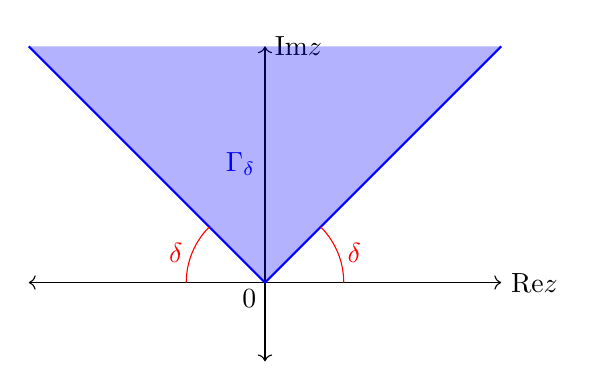
\begin{tikzpicture}[wedge/.style={blue, fill=blue, fill opacity = 0.3},
        angle/.style={red},
        axis/.style={<->,black}]
    %draw axes
    \draw[axis] (-3,0) -- (3,0) node[anchor=west]{$\text{Re} z$};
    \node at (-.2,-.2) {$0$};
    \draw[axis] (0,-1) -- (0,3) node[anchor=west]{$\text{Im} z$};
    %draw wedge
    \fill[wedge] (0, 0) -- (-3, 3) -- (3,3) -- cycle;
    \draw[thick, blue] (-3, 3) -- (0,0) -- (3,3);
    \node[left, blue] at (0,1.5) {$\Gamma_\delta$};
    %draw angle
    \def\ra{.07};
    \draw[red] (1,0) arc (0:45:1) node[midway, right]{$\delta$};
    \draw[red] (-1,0) arc (180:135:1)node[midway, left]{$\delta$};
    \end{tikzpicture}
\end{figure}
in which curves approach $0$ with an angle at least $\delta$ from the real line.

\begin{definition} (Non-Tangential Limit)
    We say $g(z) \rightarrow z_0$ non-tangentially at $z = 0$ if, for any $\delta > 0$, the limit 
    \[
        \lim_{z \rightarrow 0} g(z) = z_0
    \]
    holds for $z$ in the $\Gamma_\delta$.
    % If for any $\delta > 0$ the limit $g(z) \rightarrow L$ holds 
\end{definition}


While $g(z)$ does not generally converge at $z = 0$, in a non-tangential sense the afformentioned assymptotic expansion holds:
\begin{proposition}
\begin{enumerate}
\item If $\mu$ has bounded support
\[
    g(z) = \sum_{k = 0}^\infty c_k{(-z)}^k
\]
in a neighboorhood of $z=0$.
\item For all $n \in \NN_0$
\begin{equation}
    g(z) = \sum_{k = 0}^{n-1} c_k{(-z)}^k + z^n h_n(z) \label{assexp}
\end{equation}
where $h_n$ is such that $\lim_{z \rightarrow 0} h_n(z) = 0$ non-tangentially.
\end{enumerate}
\end{proposition}

\begin{proof}
We first note that 
\[
    \sum_{k=0}^{n} c_k {(-z)}^k 
    = \sum_{k=0}^{n} \int_{-\infty}^\infty {(-zp)}^k d\mu
    % = \int_{-\infty}^\infty \sum_{k=0}^{n} (-zx)^k d\mu
    = \int_{-\infty}^\infty \frac{1 - {(-zp)}^{n+1}}{1 + zp} d\mu
\]
and so
\begin{align*}
    h_n(z) = \frac1{z^n}\left\{g(z) - \sum_{k=0}^{n} c_k {(-z)}^k\right\}
    &= \int_{-\infty}^\infty \frac{zp^{n+1}}{1 + zp}d\mu.
\end{align*}
It remains to determine if and in what sense this trailing term $h_n(z)$ vanishes at the origin. 

As expected in the case when $\mu$ has bounded support, $h_n(z)$ exists in a neighborhood of $0$ and vanishes as $z \rightarrow 0$ in this neighboorhood. Thus the assymptotic expansion~\ref{assexp} is the Taylor expansion: The Markov transform is analytic at the origin.

When $\mu$ has unbounded support and $h_n(z)$ may not be well defined on the real line, so we must weaken our result to non-tangential convergence. If $z \in \Gamma_\delta$ then we have the following inequalities for any $p \in \RR$,
\[
    |p - z| \geq |p| \sin \delta 
    \quad\text{and} \quad
    |p - z| \geq |p| \sin \delta.
\]
We will show that
\[
    \lim_{z \rightarrow 0} h_{2n}(z) = 0, \quad z \in \Gamma_\delta
\]
from which the corresponding limit for odd orders will immediately follow from the relation
\[
    h_{2n-1}(z)
    = zh_{2n}(z) + c_{2n}z^{2n}.
\] 
Here for the sake of convenience we define $w = -\frac1z$, following a more classical approach. Note that $|w| = \frac1{|z|}$ and if $z$ is in the wedge $\Gamma_\delta$ then so is $w$. Now 
\begin{align*}
    |h_{2n}(z)| 
    &\leq \int_{-\infty}^\infty \frac{|p|^{2n+1}}{|p - w|}d\mu \\
    &\leq \frac{|z|}{\sin \delta} \int_{|p| \leq A} |p|^{2n+1} d\mu
    + \frac1{\sin \delta} \int_{|p| \geq A} p^{2n} d\mu \\
    &\leq \frac{2|z| A^{2n+2}}{\sin \delta}
    + \frac1{\sin \delta} \int_{|p| \geq A} p^{2n} d\mu
\end{align*}
Thus 
\[
    \lim_{z \rightarrow 0} |h_{2n}(z)| \leq \frac1{\sin \delta} \int_{|p| \geq A} p^{2n} d\mu, \quad z \in \Gamma_\delta.
\]
Since $A$ is arbitrary and the integral $\int p^{2n} d\mu = c_{2n}$ is convergent we are done.
\end{proof}

Evidently the assymptotic series expansion $g(z) \simeq \sum_{k=0}^\infty c_k {(-z)}^k$ is generally formal, having zero radius of convergence except in the Markov case. However as we will see in the next section, rational functions constructed from this formal series exist which approximate $g(z)$ on the upper half plane $\{\text{Im} z > 0\}$.

Finally we prove two formulas regarding the Hamburger transform of a RT projection. Let $\omega \in S^{n-1}$ be fixed and consider.
\[
    g(z) = \int_\infty^\infty \frac{R(\omega, p)}{1 + zp} dp
\]
By applying the slice theorem, with $F(p) = {(1+zp)}^{-1}$ we see that the Hamburger transform of a projection can be represented by a similar multivariable integral of $f$ over $\RR^n$.
\[
    \int_{-\infty}^\infty \frac{R_f(\omega, p)}{1 + zp} dp = \int_{\RR^n} \frac{f(x)}{1 + z\langle x, \omega \rangle} dx
\]
Similarly the GRT slice theorem with $F(p) = {(1 + zp)}^{-1}$ is
\[
    \int_{-\infty}^\infty \frac{GR_f(\omega, p) w(p)}{1 + zp} dp = \int_{\RR^n} \frac{f(x)w_n(x)}{1 + z\langle x, \omega \rangle} dx.
\]




\section{Pad\'e approximants}

In this section we recall the necessary definitions and results. Then we will prove some new results to be applied to the Gaussian Radon transform later.

\begin{definition}[Classical definition of Pad\'e approximants]
The Pad\'e approximant to a (possibly formal) power series 
\[
    R^{[L/M]}(z) \simeq \sum_{k=0}^\infty c_k z^k
\]
is a rational function with nummerator (denominator resp.) degree at most $L$ ($M$ resp.), with series equal to $\sum_{k=0}^N c_k z^k + O(z^{N+1})$ up to as high an order $N$ as possible. 
\end{definition}
Let
\[
    R^{[L/M]}(z) = \frac{P^{[L/M]}(z)}{Q^{[L/M]}(z)} = \frac{a_L z^L + \cdots + a_1z + a_0}{b_M z^M + \cdots + b_1z + b_0}.
\]
Notice that in general there is a negligable constant common factor between the numerator and denominator, so that with the remaining $L+M+1$ free parameters, we expect an order of accuracy of up to $L+M+1$ constraints, $c_0, c_1, \ldots, c_{L+M}$. Thus we define the $[L/M]$ Pad\'e approximant by the condition,
\begin{equation}
    \label{eq:BPade}
    \frac{P^{[L/M]}(z)}{Q^{[L/M]}(z)} = \sum_{k=0}^{L+M} c_k z^k + O\left(z^{L+M+1}\right).
\end{equation}
It is helpful to consider the related, and necessary condition
\begin{equation}
    \label{eq:CPade}
    P^{[L/M]}(z) = Q^{[L/M]}(z)\left(\sum_{k=0}^{L+M} c_k z^k\right) + O\left(z^{L+M+1}\right).
\end{equation}
In the classical theory of Pad\'e approximants (\ref{eq:CPade}) was often taken as a definition. It is always possible to find polynomials of the required degree satisfying this second condition, however they do not necessarily attain the degree of accuracy required by the first. We follow Baker, defining $R^{[L/M]}(z)$ by (\ref{eq:BPade}), provided such a rational function exists.

\begin{definition}
    The Pad\'e approximant $R^{[L/M]}$ to a (possibly formal) power series is a the unique rational function with nummerator (denominator resp.) degree at most $L$ ($M$ resp.) satisfying the condition (\ref{eq:BPade}). If no such rational function exists we say the Pad\'e approximant does not exist.
\end{definition}

Here we note that a sufficient condition for the equivalence of the two definitions, and hence for the existence of the Pad\'e approximant by Baker's definition is that $b_0 = Q^{L/M}(0) \neq 0$. 

Equating coeffictients of $z^k$, $k = 0, 1, \ldots, L+M$ in (\ref{eq:CPade}) gives two linear systems
\begin{align*}
    a_0 &= b_0c_0 \\
    a_1 &= b_1c_0 + b_0c_1 \\
    &\vdots \\
    a_L &= b_L c_0 + b_{L-1}c_1 + \cdots + b_0c_L
\end{align*}
and,
\begin{align*}
    0 &= b_{M}c_{L-M+1} + b_{M-1}c_{L-M+2} + \cdots + b_0c_{L+1} \\
    0 &= b_{M}c_{L-M+2} + b_{M-1}c_{L-M+3} + \cdots + b_0c_{L+2} \\
    &\vdots \\
    0 &= b_{M}c_L + b_{M-1}c_{L+1} + \cdots + b_0c_{L+M}
\end{align*}
where for convenience we set $c_k = 0$ for $k < 0$. The first systems shows the numerator $P^{[L/M]}$ is determined by the denominator $Q^{[L/M]}$. From the second system we can derive a determinantal formula for $Q^{[L/M]}$. Augmented with the desired definition, 
\[
    Q^{[L/M]}(z) = b_M z^M + b_{M-1}z^{M-1} + \cdots + b_0
\]
the system can be written in the form
\[
    \begin{pmatrix}
        0 \\ 0 \\ \vdots \\ 0 \\ Q^{[L/M]}(z)
    \end{pmatrix}
    =
    \begin{pmatrix}
        c_{L-M+1} & c_{L-M+2} & \cdots & c_{L+1} \\
        c_{L-M+2} & c_{L-M+3} & \cdots & c_{L+2} \\
        \vdots & \vdots & \ddots & \vdots \\
        c_{L} & c_{L+1} & \cdots & c_{L+M} \\
        z^M & z^{M-1} & \cdots & 1
    \end{pmatrix}
    \begin{pmatrix}
        b_M \\ b_{M-1} \\ \vdots \\ b_1 \\ b_0
    \end{pmatrix}
\]
Solving for $b_0$ by Cramer's Rule we get,
% \[
%     b_0 = 
%     \frac{
%         \left|
%         \begin{matrix}
%             c_{L-M+1} & c_{L-M+2} & \cdots & c_L & 0 \\
%             c_{L-M+2} & c_{L-M+3} & \cdots & c_{L+1} & 0 \\
%             \vdots & \vdots & \ddots & \vdots & \vdots \\
%             c_L & c_{L+1} & \cdots & c_{L+M-1} & 0 \\
%             z^M & z^{M-1} & \cdots & z & Q^{[L/M]}(z)
%         \end{matrix}
%         \right|
%     }{
%         \left|
%         \begin{matrix}
%             c_{L-M+1} & c_{L-M+2} & \cdots & c_{L+1} \\
%             c_{L-M+2} & c_{L-M+3} & \cdots & c_{L+2} \\
%             \vdots & \vdots & \ddots & \vdots \\
%             c_{L} & c_{L+1} & \cdots & c_{L+M} \\
%             z^M & z^{M-1} & \cdots & 1
%         \end{matrix}
%         \right|
%     }
% \]

% \[
%     b_0 = 
%     \frac{
%         \left|
%         \begin{matrix}
%             c_{L-M+1} & c_{L-M+2} & \cdots & c_L \\
%             c_{L-M+2} & c_{L-M+3} & \cdots & c_{L+1} \\
%             \vdots & \vdots & \ddots & \vdots  \\
%             c_L & c_{L+1} & \cdots & c_{L+M-1} 
%         \end{matrix}
%         \right| Q^{[L/M]}(z)
%     }{
%         \left|
%         \begin{matrix}
%             c_{L-M+1} & c_{L-M+2} & \cdots & c_{L+1} \\
%             c_{L-M+2} & c_{L-M+3} & \cdots & c_{L+2} \\
%             \vdots & \vdots & \ddots & \vdots \\
%             c_{L} & c_{L+1} & \cdots & c_{L+M} \\
%             z^M & z^{M-1} & \cdots & 1
%         \end{matrix}
%         \right|
%     }
% \]

\[
    b_0
    \left|
    \begin{matrix}
        c_{L-M+1} & c_{L-M+2} & \cdots & c_{L+1} \\
        c_{L-M+2} & c_{L-M+3} & \cdots & c_{L+2} \\
        \vdots & \vdots & \ddots & \vdots \\
        c_{L} & c_{L+1} & \cdots & c_{L+M} \\
        z^M & z^{M-1} & \cdots & 1
    \end{matrix}
    \right|
    =
    \left|
    \begin{matrix}
        c_{L-M+1} & c_{L-M+2} & \cdots & c_L \\
        c_{L-M+2} & c_{L-M+3} & \cdots & c_{L+1} \\
        \vdots & \vdots & \ddots & \vdots  \\
        c_L & c_{L+1} & \cdots & c_{L+M-1} 
    \end{matrix}
    \right| 
    Q^{[L/M]}(z)
\]
The LHS is clearly a polynomial, and nonzero if the RHS minor is nonzero. Thus if the Hankel determinant
\[
    \left|
    \begin{matrix}
        c_{L-M+1} & \cdots & c_L \\
        \vdots & \ddots & \vdots  \\
        c_L & \cdots & c_{L+M-1} 
    \end{matrix}
    \right| 
\]
is nonzero, then up to the afformentioned constant factor,
\begin{equation}
    Q^{[L/M]}(z) = 
    \left|
    \begin{matrix}
        c_{L-M+1} & \cdots & c_{L+1} \\
        \vdots & \ddots & \vdots \\
        c_{L} & \cdots & c_{L+M} \\
        z^M & \cdots & 1
    \end{matrix}
    \right| 
    \label{eq:Qdet}
\end{equation}
By convention we normalize $R^{[L/M]}(z)$ so that $b_0 = Q^{[L/M]}(0) = 1$. 

Since the Hankel determinants give a useful form for expressing some conditions of interest we will difine $H(n,m)$ to be the determinant of the $(m + 1) \times (m + 1)$ Hankel matrix starting with $c_n$,
\[
    H(n,m) :=
    \left|
    \begin{matrix}
        c_{n} & \cdots & c_{n+m} \\
        \vdots & \ddots & \vdots  \\
        c_{n+m} & \cdots & c_{n+2m} 
    \end{matrix}
    \right|
\]
Note in particular that the sufficient condition $Q^{[L/M]}(0) \neq 0$ for the existence of $R^{[L/M]}(z)$ is equivalent to $H(L-M+1, M-1) \neq 0$

We now narrow our focus to Pad\'e approximants to a Humburger series. Let $\mu$ be a Borel measure on $\RR$ with infinite support and finite moments $c_k = \int p^k ~d\mu$. Recall that the Hamburger transform of $\mu$,
\[
    g(z) := \int_\RR \frac{d\mu}{1+pz}
\]
has the assymptotic expansion, in the sense of non-tangential limits,
\[
    g(z) \simeq \sum_{k=0}^\infty c_k (-z^k).
\]
We call this formal power series a Hamburger series. 

\begin{remark}
    \tc{To simplify the rest of this maybe we redefine}
    \[
        c_k = {(-1)}^k\int p^k d\mu
    \]
\end{remark}

\begin{lemma}
    The hamburger moments $c_k$ satisfy the determinental condition $H(2n, m) \neq 0$ for $n,m = 0, 1, \ldots$. 
\end{lemma}
\begin{proof}
    Consider the quadratic form given by
    \[
        G(\mathbf{x}, \mathbf{y}) := 
        \mathbf{x}^\top
        \begin{pmatrix}
            c_{2n} & \cdots & c_{2n+m} \\
            \vdots & \ddots & \vdots  \\
            c_{2n+m} & \cdots & c_{2n+2m}
        \end{pmatrix}
        \mathbf{y}
    \]
    If $\mathbf{x} = {(x_0, x_1, \ldots, x_m)}^\top$ then
    \begin{align*}
        G(\mathbf{x}, \mathbf{x})
        &= \sum_{i,j=0}^m x_i x_j c_{2n+i+j} \\
        &= \sum_{i,j=0}^m x_i x_j \int p^{2n+i+j} ~d\mu \\
        &= \int \sum_{i,j=0}^m x_i x_j p^{2n+i+j} ~d\mu \\
        &= \int p^{2n} {\left(\sum_{k=0}^m x_k p^{k}\right)}^2 ~d\mu 
        \geq 0.
    \end{align*}
    Thus $G(\mathbf{x}, \mathbf{y})$ is positive semi-definite. Furthermore, equality holds
    \[
        \int p^{2n}{\left(\sum_{k=0}^m x_k p^{k}\right)}^2 ~d\mu = 0
    \]
    if and only if $\mu$ is supported entirely on the zeros of the polynomial $p^n\sum_{k=0}^m x_k p^{k}$. However by assumption $\mu$ has infinite support. So in fact $G$ is strictly positive definite. We conclude, by Sylvester's criterion for example, that assocciated hankel matrix has positive determinant. That is, $D(2n, m) > 0$.
\end{proof}

The previous lemma guarentees the existence of certain Pad\'e approximants, specifically those with $L-M+1$ even. 
\begin{theorem}
    If $J$ is odd then the Pad\'e approximant $R^{[L/L+J]}(z)$ to the Hamburger series exists in Baker's sense.
\end{theorem}

% Following Baker's definition [Baker] we say the Pad\'e approximant $R^{[L/M]}$ exists if it satisfies this order of accuracy condition. For details on the construction of Pad\'e approximants see [Baker], []. When the formal series is arbitrary one cannot guarentee the existence of any given $R^{[L/M]}$. However as we will see the situation for Pad\'e approximants to a Hamburger series, for which much is known from the classical theory of moment problems and orthogonal polynomials, is much nicer than the greneral theory.

With our particular application in mind, we will assume the measure $\mu$ is absolutely continuous with respect to the Lebesgue measure and denote it $f(x)dx$ where $f(x)$ is some non-negative Lebesgue measureable function of $\RR$. Let $R_M(z)$ be the ``offdiagonal'' approximant $R^{[M/M+1]}(z)$ to the Hamburger series of $\mu$,
\[
    R_M(z) = \frac{P_M(z)}{Q_M(z)} \approx \sum_{k=0}^\infty c_k {(-z)}^k \simeq \int_{-\infty}^\infty \frac{f(p)}{1 + zp} ~dp
\]
where $c_k = \int p^k f(p) dp$. In this section we will prove

\begin{theorem}
    The off-diagonal Pad\'e approximants $R_M(z)$ to the a determinate Hamburger series $\sum_{k=0}^\infty c_k {(-z)}^k$ exist and converge to $g(z)$ uniformly on compact subsets of the upper half plane $\{\text{Im} ~z > 0\}$.
\end{theorem}

An outline of the proof is as follows: We first justify that the approximants exist in Baker's sense. Then it can be shown that limit of any convergent subsequence of $R_M$ must have a representation as the Hamburger transform of some Borel measure $\mu$ which is a solution to our moment problem, and that furthermore such convergent subsequences exist. Thus in order for the sequence $R_M$ to converge to $g(z)$ it will be necessary and sufficient that the moment problem be determinate.

% Convergence $R_M(z) \rightarrow g(z)$ is \tc{related in some way cant remember} to the determinacy of the moment problem for the sequence $\{c_k\}$. Recall that a moment problem is called determinate if it has a unique solution. \tc{In Akheizer's world, if the moment problem is determinate, then $w_\infty(z)$ is a point for all $z$. Each $R_M$ coresponds to a point $w_M(\omega) = \frac1\omega R_m(-\frac1\omega)$. The points $w_M$ must converge to $w_\infty$}

\begin{proposition}
    If the sequence $c_k$ gives a determinate moment problem then the off-diagonal Pad\'e approximants $R_M(z)$ converge to $g(z)$ locally uniformly.
\end{proposition}

\begin{proof}
    The Pad\'e approximant $R_M(z)$ has a convenient representation as an inner product in terms of a finite Jacobi matrix,
    \[
        R_M(z) = \langle \delta_0, {(1 + zA_M)}^{-1} \delta_0 \rangle.
    \]
    Now since $A_M$ is a real matrix and $\frac1{|w|} \geq \frac1{|\text{Im}(w)|}$ for any $w \in \CC$, we see that
    \[
        |zR_M(z)| = |\langle \delta_0, {(z^{-1} + A_M)}^{-1} \delta_0 \rangle| \leq \frac1{|\text{Im}(1/z)|}
    \]
    and thus
    \[
        |R_M(z)| \leq \frac1{|z||\text{Im}(1/z)|} = \frac{|z|}{|\text{Im}(z)|}.
    \]
    Since this bound is independent of $R_M$, Montel's theorem implies that the off-diagonal Pade approximants form a normal family. It can be shown that the limit of any convergent subsequence has a representation $\int (1+ xz)d\sigma(x)$ where $\sigma$ is a solution to the Hamburger moment problem. Since the moment problem is determinate, the sequence $R_M$ must converge to $g(z)$ uniformly on compact sets.
\end{proof}

It remains to discuss the determinacy of the Hamburger moment problem. Here we need to add an additional constraint on the measure $d\mu = f(p)dp$, which is that $f(p)$ is $L^2$ integrable with respect to the Gaussian weight.

\begin{proposition}
    A function $f(p) \in L^2(\mathbb{R}, e^{-p^2}dp)$ such that the moments 
    \begin{equation}
        \label{eq:3}
        c_k = \int_{-\infty}^\infty p^k f(p) e^{-p^2} ~dp, ~ k = 0, 1 \ldots
    \end{equation}
    are finite, is uniquely determined by those moments.
\end{proposition}
    
\begin{proof}
    It is sufficient to show that if $c_k = 0$ for all $k \geq 0$, then $f \equiv 0$ a.e. The Hermite moments are just linear combinations of $0$,
    \[
        \int_{-\infty}^\infty H_k(p) f(p) e^{-p^2} ~dp = 0, ~ k \geq 0
    \]
    where $H_k(p)$ is the Hermite polynomial of order $k$. Since the Hermite polynomials are complete in the space $L^2(\mathbb{R}, e^{-p^2}dp)$ then $f \equiv 0$.
\end{proof}





% % \begin{figure}
% %     \centering
% %     \begin{tikzpicture}
% %         \draw[->] (0, 0) -- (5, 0) node[right] {$x$};
% %         \draw[->] (0, 0) -- (0, 1) node[above] {$y$};
% %         \draw[scale=0.5, domain=1:5, smooth, variable=\x, blue] plot ({\x}, {\x  *exp(-ln(\x))});
% %     \end{tikzpicture}
% % \end{figure}


% Given a formal power series $g(z) = \sum_{k=0}^\infty c_kz^k$ the Pad\'e approximant of degree $[L/M]$ is a rational function whose series expansion agrees with that of $g(z)$ as much as possible, which we denote by $[L/M]_g = \frac{P^{[L/M]}}{Q^{[L/M]}}$ where $P^{[L/M]}(z) = \sum_{k=0}^L a_kz^k$ and $Q^{[L/M]}(z) = \sum_{k=0}^M b_kz^k$ are polynomials of degree at most $L$ and $M$ respectively.  
% \begin{equation}
%     \label{eq:pade}
%     g(z) = [L/M]_g(z) + O(z^{N_{[L/M]}})
% \end{equation}
% Counting unknown coefficients, we can expect an order of accuracy of at most $N_{[L/M]} = L+M+1$. More precisely, we cross multiply and consider the related condition,
% \begin{equation}
%     \label{eq:cross}
%     Q^{[L/M]}(z)g(z) - P^{[L/M]}(z) = O(z^{L+M+1}),
% \end{equation}
% which can be written as a system of $L + M + 1$ linear equations
% \begin{align*}
%     \sum_{\ell = 0}^k b_\ell c_{k-\ell} &= a_k & k &= 0, 1, \ldots, L \\
%     \sum_{\ell = 0}^k b_\ell c_{k-\ell} &= 0, & k &= L + 1 \ldots, L + M
% \end{align*}
% where for convenience we set $b_\ell = 0$, $\ell > M$ and $c_\ell = 0$, $\ell < 0$. Thus a solution $b_0, \ldots, b_M$ can be found to a underdetermined homogeneous system of $M$ equations in $M+1$ unknowns, and then $a_0, \ldots, a_L$ can be computed directly. The rational function $\frac{P^{[L/M]}}{Q^{[L/M]}}$ has an irreducible form $\frac{P_\star^{[L/M]}}{Q_\star^{[L/M]}}$ which can be normalized so that $Q_\star^{[L/M]}(0) = 1$. Subject to these constraints this defines a unique rational approximation satisfying (\ref{eq:cross}) and from now the notation $[L/M]_g$ will refer to the unique normalized irreducible form $\frac{P_\star^{[L/M]}}{Q_\star^{[L/M]}}$. Note that $[L/M]_g$ computed in this way may not satisfy (\ref{eq:pade}) up to the desired order $L+M+1$, particularly in the case when $Q^{[L/M]}(0)=0$. In the event that no rational function of degree $[L/M]$ exists approximating $g$ to the desired accuracy we say the $[L/M]$ Pad\'e approximant does not exist. We will focus on cases where they do exist. Besides, in general it can be shown that infinitely many approximants exist in a sense in which we can move on to talking about convergence.

% The convergence of Pad\'e approximants is  not fully understood in general. We will concern ourselves with a particular case for which these questions have answers: approximants on a diagonal, $[m+k/m]$ as $m \rightarrow \infty$ for certain integral forms.


% Now consider the function defined by
% \[
%     g(z) = \int_{-\infty}^\infty \frac{GR_f(\omega, p)e^{-p^2}}{1 - zp} ~dp
% \]
% which has an at least formal expansion
% \[
%     g(z) \simeq \sum_{n=0}^\infty c_kz^k
% \]
% where
% \[
%     c_k = \int_{-\infty}^\infty p^k GR_f(\omega, p)e^{-p^2} ~dp.
% \]

% In this case question of the convergence $[L/M]_g \rightarrow g$ is related to whether this Hamburger moment problem is determinate.
% \begin{proposition}
% A function $f(p) \in L^2(\mathbb{R}, e^{-p^2}dp)$ such that the moments 
% \begin{equation}
%     \label{eq:3}
%     c_k = \int_{-\infty}^\infty p^k f(p) e^{-p^2} ~dp, ~ k = 0, 1 \ldots
% \end{equation}
% are finite, is uniquely determined by those moments.
% \end{proposition}

% \begin{proof}
%     It is sufficient to show that if $c_k = 0$ for all $k \geq 0$, then $f \equiv 0$ a.e. The Hermite moments are just linear combinations of $0$,
% \[
%     \int_{-\infty}^\infty H_k(p) f(p) e^{-p^2} ~dp = 0, ~ k \geq 0
% \]
% where $H_k(p)$ is the Hermite polynomial of order $k$. Since the Hermite polynomials are complete in the space $L^2(\mathbb{R}, e^{-p^2}dp)$ then $f \equiv 0$.
% \end{proof}

% \tc{My understanding here is that since the moments $c_k$ uniquely determine $GR_f(\omega, p)$, and thus $g(z)$, then the Pad\'e approximants, if they converge, must converge to $g(z)$. Correct?}


% We will now (attempt to) define a multivariate analogue to the Pad\'e approximants. We'll detail the bivariate case for example and promise that higher dimensions follow similarly. Informally, a multivariate power series is written as a sum of homogeneous polynomials, the Pad\'e approximants similarly decomposed into homogeneous polynomials. A system of linear equations is formed nearly identical to that of the classical Pad\'e approximants, but with somewhat more unknowns. A "degree shift" by $LM$ is necessary to ensure the system has a nontrivial solution. According to Cuyt the structure of this system (so called "near Toeplitz") reduces the complexity for computing solutions from $O(n^3)$ to $O(\alpha n^2)$ where $n$ is the dimension of the system and $\alpha$ is its "displacement rank." As in the univariate case it is shown these Pad\'e approximants have a unique reduced form up to a normalization constant.

% \tc{I obviously need to fill in a lot more detail here. The "degree shift" is currently what is confusing me...}

% Let me be more specific... \tc{use multi-index notation? Probably not necessary, but it looks cleaner.} Consider a formal power series in the variable $x = (x_1, \ldots, x_d) \in \mathbb{R}^d$
% \[
%     g(x) = \sum_{\alpha_1, \ldots, \alpha_d = 0}^\infty c_{\alpha_1, \ldots, \alpha_d} x_1^{\alpha_1}\cdots x_d^{\alpha_d} = \sum_{\ell = 0}^\infty C_\ell(x)
% \]
% where $C_\ell(x^\ell)$ is a homogeneous polynomial in the coordinates of $x$,
% \[
%     C_\ell(x) := \sum_{\alpha_1 + \cdots + \alpha_d = \ell} c_{\alpha_1, \ldots, \alpha_d} x_1^{\alpha_1}\cdots x_d^{\alpha_d}.
% \]
% Similarly to the univariate case we seek a rational function $[L/M]_g = \frac{P^{[L/M]}}{Q^{[L/M]}}$ where
% \[
%     P^{[L/M]}(x) 
%     % = \sum_{|\alpha| \leq L} a_\alpha x^\alpha
%     = \sum_{\ell = LM}^{LM + L} A_\ell(x)
%     = \sum_{\ell = LM}^{LM + L} \sum_{|\alpha| = \ell} a_\alpha x^\alpha
% \]
% \[
%     Q^{[L/M]}(x) 
%     % = \sum_{|\alpha| \leq M} b_\alpha x^\alpha
%     = \sum_{\ell = LM}^{LM + M} B_\ell(x)
%     = \sum_{\ell = LM}^{LM + M} \sum_{|\alpha| = \ell} b_\alpha x^\alpha
% \]
% such that
% \[
%     g(x) = [L/M]_g(x) + O(x^\alpha, |\alpha| \geq LM + L + M + 1).
% \]
% Note the "degree shift" by $LM$, which is necessary to guarantee nontrivial solutions. Following the univariate case we cross multiply and consider the accuracy through order condition
% \begin{equation}
%     \label{eq:multicross}
%     Q^{[L/M]}(x)g(x) - P^{[L/M]}(x) = O(z^{LM + L+M+1}),
% \end{equation}
% which once again gives $Q^{[L/M]}(x)$ as a solution to an underdetermined (because of the degree shift) homogeneous system of linear equations, and $P^{L/M}(x)$ is computed from the remaining equations. 

% A useful note about the homogeneous form for the power series, which we will use later, is that when restricted to the slice $x = p\omega$ for a fixed unit vector $\omega \in \mathbb{R}^n$ it is easily expressed as a power series in $p$,
% \[
%     \sum_{\ell = 0}^\infty C_\ell(p\omega)
%     = \sum_{\ell = 0}^\infty C_\ell(\omega) p^\ell
% \]
% and similarly for the polynomials.
% \tc{[Note to self and Maxim] This seems to be the crux of the "powerful slice theorem" for homogeneous Pad\'e approximant (Cuyt's Theorem 2). The degree shift, which just adjusts the dimensions of the linear system to guarantee a nontrivial solution, reduces on slices: if $P^{[L/M]}(x) = \sum_{\ell = LM}^{LM+L}A_\ell(x)$, $Q^{[L/M]}(x) = \sum_{\ell = LM}^{LM+M} B_\ell(x)$ then
% \[
%     \frac{P^{[L/M]}(p\omega)}{Q^{[L/M]}(p\omega)}
%     = \frac{\sum_{\ell = LM}^{LM+L}A_\ell(\omega)p^{\ell}}{\sum_{\ell = LM}^{LM+M}B_\ell(\omega)p^{\ell}}
%     = \frac{\sum_{\ell = 0}^{L}A_{LM+\ell}(\omega)p^\ell}{\sum_{\ell = 0}^{M}B_{LM+\ell}(\omega)p^\ell}
% \]
% the RHS satisfies the "accuracy through order condition" (\ref{eq:cross})... 
% \begin{align*}
%     \left(\sum_{\ell=0}^\infty C_{\ell}(\omega)p^\ell\right)
%     \left(\sum_{\ell=0}^M B_{LM+\ell}(\omega)p^\ell\right) -
%     \sum_{\ell=0}^L A_{LM+\ell}(\omega)p^\ell \\
%     = \frac1{p^{LM}} \left(g(p\omega) Q^{[L/M]}(p\omega) - P^{[L/M]}(p\omega)\right)
%     = O(p^{L+M+1})
% \end{align*}
% and thus in irreducible form is equal to the unique univariate Pad\'e approximant for $g_\omega(p) := g(p\omega)$. On a personal note it is so much clearer to write this out with the general degree $[L/M]$ as opposed to $[m + k/m]$. The proof above would work for any degree shift, so long as the multivariate pade order through accuracy condition is satisfied.}

% \tc{...insert the construction of multi pade}

\section{Convergence results for the Gaussian Radon transform}
% What is the relationship between the Gaussian and Classical Radon Transform
% \[
%     GR_f(\omega, p)e^{-p^2/2} 
%     = e^{-p^2/2} \int_{\langle x, \omega \rangle = p} e^{-|p\omega-x|^2/2} f(x) dx
%     = \int_{\langle x, \omega \rangle = p} e^{-|x|^2/2} f(x) dx
%     = R_g(\omega, p)
% \]
% where $g(x) = e^{-|x|^2/2} f(x)$

% \begin{tikzcd}
%     f \arrow[d, "\psi"] \arrow[r, "\eta"]
%     & Gf \arrow[d, "\psi"] \\
%     R_f \arrow[r, "\eta"]
%     & GR_f
% \end{tikzcd}



Now we are in the position to assemble all the previous results into an approximation scheme to be used for reconstruction shapes of unbounded domains.

Take a non-negative Lebesgue measureable function $f(x)$ on $\RR^n$ with finite multivariate Gaussian moments
\[
    c^G_\alpha = \int_{\RR^n} f(x)e^{-\|x\|/2} x^\alpha dx
\]
We have seen that the multivariate Stieltjes transform of $f$, 
\[
    g(z) = \int_{\RR^n} \frac{f(x)e^{-\|x\|/2}}{1 + \langle x, \omega \rangle z} dx,
\]
is equal to the Hamburger transform of $GR_f(\omega, p)$, whose moments in turn are easily computed from the moments of $f$, for fixed $\omega$. Thus for $z$ in the one dimensional subspace spanned by $\omega$, $g(z)$ can be approximated well by Pad\'e approximants, under the integrability condition $GR_f(\omega, p) \in L^2(\RR, e^{-p^2}~dp)$. On the other hand as an integral on $\RR^n$, we can also approximate $g(z)$ by cubature formula,
\[
    \int_{\RR^n} \frac{f(x)e^{-\|x\|^2/2}}{1 + \langle x, \omega \rangle z} dx 
    \approx \sum_{\ell = L} \frac{e^{-\|x_\ell\|^2/2}}{1 + \langle x_\ell, \omega \rangle z} w_\ell f(x_\ell)
    =: \sum_{\ell = L} C_\ell(z) f(x_\ell).
\]
By equating these parallel approximations, 
\[
    \sum_{\ell = L} C_\ell(z) f(x_\ell) \approx R_M(z),
\]
with a sufficient quantity of sample points $z_j$ we have arrived at a linear system
\[
    \sum_{\ell = L} C_\ell(z_j) f(x_\ell) = R_M(z_j), 
    \qquad j = 1, 2, \ldots, J
\]
from which we should be able to recover the value of $f$ on our cubature nodes $x_\ell$.



% We have seen that the Hamburger transform of the GRT of $f$,
% \[
%     g(z) = \int_{-\infty}^\infty \frac{GR_f(\omega, p) e^{-p^2/2}}{1 + pz}dp
% \]
% can be approximated to an arbitrary degree by offdiagonal Pad\'e approximants, $R_M(z)$ near zero. On the other hand as an integral over $p$

\section{Implementation}

While the authors describe forming multivariate ``homogeneous'' Pade approximants — perhaps first proposed by Cuyt herself in~\cite{Cuyt84} — we opt to bypass this step using univariate approximants instead. Indeed, the only benefit to Cuyt's approximants explicitly cited by the authors, as compared to other multivariate generalizations of the Pade approximants, is that they are ``the only satisfying the following powerful slice theorem''~\cite{Cuyt05}. This slice theorem simply states that the homogeneous approximants when restricted to one dimensional subspaces, are equivalent to univariate Pade approximants. Since we only need a finite number of sample points it seems reasonable to compute a series of univariate approximants at various projection angles.

The decision to drop the homogenous approximants has the following potential consequences: On the one hand, the univariate approximants are simpler to compute, with methods built in to many CASs. On the other, while the authors select sample points from a cubic lattice, it would be inefficient (though potentially less so with careful selection of projection angles via, say, Farey sequences) to do so with one dimensional subspaces. Instead we take a collection of equidistant projection angles forming a radial grid of sample points. This seems acceptable, as it is unclear if there is any benefit to the sample points having a particular geometric structure. We should also agknowledge the potential that forming a single homogeneous appoximant is more computationally efficient than many univariate approximants. This requires further investigation, but we note that (anecdotally) in computational tests the formation of approximants is not very intensive compared to the subsequent solving of the high dimensional linear system. Some thought was given to the possibility that sampling from a cubic lattice provides some structure which makes the system easier to solve, but so far we have no hard evidence of this.

A couple of notes on computational details: First we should be explicit about the line of computation. At the outset, the given information is a certain multivariate moment sequence (up to a finite order with some accuracy assumption) which we assume belongs to a region within some fixed bounding box. In evaluating the computational viability of the method we take note of which steps depend on the moments, and which can be precomputed. In order to form univariate approximants we first compute projection moments. While these of course depend on the moment sequence, the multinomial formula used for this computation only depends on the projection angle. Thus with a preditermined set of projection angles this is partially precomputed. Since the cubature formula itself only depends on the choice of quadrature nodes and sample points, it can be precomputed and applied to any moment sequence. The choice of quadrature formula is somewhat arbitrary. Lacking expertise in the area of numerical integration, we follow the authors, opting for the four-point Gauss-Legendre product formula. This formula takes nodes from a nearly cubic lattice, which is implicitly quantized when forming the pixel image. We have not evaluated the error introduced by this quantization but expect it to be minimal and to approach zero with higher pixel resolution.

We don't expect the linear system to have an exact solution, let alone one that whose computation is tractable for high resolutions. We may try Mathematica's LeastSquares method, but Cuyt et al.\ specifically mention using a truncated singular value decomposition.

For my own benefit, let's review singular value decompositions. An $i \times j$ matrix $A$ of rank $r$ can be written as 
\[
    A=U\Sigma V^\top,
\]
where $\Sigma$ is the diagonal matrix of singular values $\sigma_1, \sigma_2, \ldots, \sigma_r$, and $U$ and $V$ are unitary matrices. The truncated singular value decomposition gives us a reduced rank approximation to $A$ by replacing all but the largest (first) $k$ singular values in $\Sigma$ with zeros,
\[
    \tilde{\Sigma} = \text{diag}(\sigma_1, \sigma_2, \ldots, \sigma_k, 0, \ldots, 0)
\] 
The truncated SVD matrix $\tilde{A} = U \tilde{\Sigma} V^\top$ is optimal in the sense that it is the closest rank-$k$ matrix to $A$ in the Frobenius norm.

The SVD and truncated SVD are used to solve the linear least squares problem as follows: From $U\Sigma V^\top f = p$ we get $f=V \Sigma^{-1} U^\top p$, and similarly $f = \tilde{V} \tilde{\Sigma}^{-1} U^\top p$. Note that the psuedoinverse $\tilde\Sigma^{-1}$ is a diagonal matrix made up of the reciprocal singular values.

Mathematica offers a few built in functions for this. LeastSquares packages a number of methods to solve a linear least squares based on the sparsity of the System (our system is dense). SingularValueDecomposition can be restricted to a certain number of singular values. PsuedoInverse can specify a ``tolerance'' zeroing out singular values less than some proportion of  the maximum singular value. While LeastSquares is the simplest option, it does not seem to support truncated solutions. Between SingularValueDecomposition and PsuedoInverse, both can handle truncated problems, but the latter seems — at least superficially — better suited for out application.

On Gaussian shape reconstruction. There remain some minor practical concerns about, for example, the choice of quadrature formula and sample points. An obvious choice would be to continue with the Gauss-Legendre product formula, now applied on a Gaussian-weighted $f$. Some consideration should be taken as to the viability of other Gaussian quadrature formulas defined particulary for the Gaussian measure. 

Now, a fundamental limitation with the proposed method which we have neglected to mention is the practical one: As a computational method we are necessarily restriced to the finite — finite moments, finite order approximations, and most problamatic, bounded domains. In what application would one even be interested in unbounded shape reconstruction, while also having access of Gaussian moments? It would be reasonable to question the use of a computational method in an unbounded context. As with any finite approximation, the unboundedness should be thought of as an idealized limit; perhaps an unbounded approximation is a limit of bounded approximations. But then, the original method applies just as well if all we wanted was a sequence of reconstructions expanding in range. We can only speculate at this point that perhaps this method, being taylored specifically for unbounded reconstruction, could hold some practical advantages over its predecessor; or be satisfied with impracticality.

\section{An example}

% \[
%     w(x) = w_1(x) = \frac1{\sqrt{2\pi}}e^{-\frac{x^2}2}
% \]
% \[
%     w_2(x, y) = \frac1{2\pi}e^{-\frac{x^2 + y^2}2}
% \]

\[
    f : \RR^2 \rightarrow \RR
\]
\begin{align*}
    GR_f(\theta, p) 
    &= \int_{-\infty}^\infty f(x(t), y(t)) w(t)~dt \\
    &= \int_{-\infty}^\infty f(t \sin\theta + p \cos\theta, -t \cos\theta + p \sin\theta) w(t)~dt
\end{align*}

% Let $f_{i,j} = x^i y^j$ for $i, j \in \NN_0$. Define $G_{i,j}(\theta, p) = GR_{f_{i,j}}(\theta, p)$
% \[
%     G_{i,j}(\theta, p)
%     = \frac1{\sqrt{2\pi}}\int_{-\infty}^\infty {(t \sin\theta + p \cos\theta)}^i {(-t \cos\theta + p \sin\theta)}^j e^{-\frac{t^2}2}~dt
% \]
% In particular 
% \begin{align*}
%     G_{0,0}(\theta, p) 
%     &= 1 \\
%     G_{1,0}(\theta, p) 
%     &= \frac1{\sqrt{2\pi}}\int_{-\infty}^\infty (t \sin\theta + p \cos\theta) e^{-\frac{t^2}2}~dt
% \end{align*}

Let $H_\alpha(x) = H_{\alpha_1}(x_1)H_{\alpha_2}(x_2) \cdots H_{\alpha_n}(x_n)$ for $\alpha \in \NN_0^n$ and when $n=2$,
\[
    H_{i,j}(x,y) = H_i(x)H_j(y)
\]
Mathematica table: $\frac{GR_{H_{i,j}}(\theta,p)}{\cos^i\theta \sin^j\theta}$ for $i,j \leq 4$
\[
\begin{array}{ccccc}
 1 & p & p^2-1 & p^3-3 p & p^4-6 p^2+3 \\
 p & p^2-1 & p^3-3 p & p^4-6 p^2+3 & p^5-10 p^3+15 p \\
 p^2-1 & p^3-3 p & p^4-6 p^2+3 & p^5-10 p^3+15 p & p^6-15 p^4+45 p^2-15 \\
 p^3-3 p & p^4-6 p^2+3 & p^5-10 p^3+15 p & p^6-15 p^4+45 p^2-15 & p^7-21 p^5+105 p^3-105 p \\
 p^4-6 p^2+3 & p^5-10 p^3+15 p & p^6-15 p^4+45 p^2-15 & p^7-21 p^5+105 p^3-105 p & p^8-28 p^6+210 p^4-420 p^2+105 \\
\end{array}
\]

\textbf{Conjecture:} Based on a Mathematica table (at least up to $i,j\leq4$) it seems that the following formula holds:
\[
    GR_{H_{i,j}}(\theta, p) = H_{i+j}(p) \cos^i \theta \sin^j \theta 
\]
We further expect 
\[
    GR_{H_\alpha}(\omega, p) = H_{|\alpha|}(p) \omega^\alpha
\]
for $\alpha \in \NN_0^n$.

Bogachev: $(H_\alpha)_{\alpha \in \NN_0^n}$ is an orthogonal basis in $L^2(\gamma_n)$

Mathematica table: $GR_f(a, p)$ for $f(x,y) = x^i y^i$
\[
\begin{array}{cccc}
    1 & p \sin (a) & p^2 \sin ^2(a)+\cos ^2(a) & p \sin (a) \left(p^2 \sin ^2(a)+3 \cos ^2(a)\right) \\
    p \cos (a) & \left(p^2-1\right) \sin (a) \cos (a) & p \cos (a) \left(\left(p^2-2\right) \sin ^2(a)+\cos ^2(a)\right) & \sin (a) \cos (a) \left(p^2 \left(p^2-3\right) \sin ^2(a)+3 \left(p^2-1\right) \cos ^2(a)\right) \\
    p^2 \cos ^2(a)+\sin ^2(a) & p \sin (a) \left(\left(p^2-2\right) \cos ^2(a)+\sin ^2(a)\right) & \frac{1}{8} \left(-\left(p^4-6 p^2+3\right) \cos (4 a)+p^4+2 p^2+3\right) & \frac{1}{8} p \sin (a) \left(8 \left(p^2-3\right) \cos (2 a)-\left(p^4-10 p^2+15\right) \cos (4 a)+p^4+6 p^2-9\right) \\
    p \cos (a) \left(p^2 \cos ^2(a)+3 \sin ^2(a)\right) & \frac{1}{4} \sin (2 a) \left(\left(p^4-6 p^2+3\right) \cos (2 a)+p^4-3\right) & \frac{1}{8} p \cos (a) \left(-8 \left(p^2-3\right) \cos (2 a)-\left(p^4-10 p^2+15\right) \cos (4 a)+p^4+6 p^2-9\right) & \frac{1}{16} \sin (2 a) \left(-\left(p^6-15 p^4+45 p^2-15\right) \cos (4 a)+p^6+9 p^4-27 p^2-15\right) \\
    \end{array}
\]

\[
    f(x) =
    \begin{cases}
        1, & \langle x, \varphi \rangle \leq 1/2 \\
        0, & \text{otherwise}
    \end{cases}
\]

Unit ball in $\RR^3$? Annulus in $\RR^2$? Some assymmetric or off-center examples?



\bibliography{references}
\end{document}
